\chapter{Introducción}
\label{chap1}
\ifpdf
  \graphicspath{{Chapter1/Chapter1Figs/PNG/}{Chapter1/Chapter1Figs/PDF/}{Chapter1/Chapter1Figs/}}
\else
  \graphicspath{{Chapter1/Chapter1Figs/EPS/}{Chapter1/Chapter1Figs/}}
\fi

\markboth{\hfill \thechapter. Introducción}{\hfill \thechapter. Introducción}

El impacto ambiental que provocan los residuos sólidos municipales ha sido objeto de atención especial en las últimas décadas. La eliminación de los residuos sólidos urbanos es una preocupación creciente en todo el mundo, sin importar el tamaño ni las características socio-económicas de una ciudad. Muchas ciudades se han visto obligadas a evaluar su programa de gestión de residuos sólidos y examinar su relación costo-efectividad en términos de recolección, transporte, tratamiento y eliminación \citep{Karadimas2007OptimalAlgorithm}.

Según la literatura, los sistemas de gestión de basura estiman que de la cantidad total de dinero gastado para la recogida, transporte y eliminación de residuos sólidos, aproximadamente el 60-80\% se gasta en la fase de recogida. Por ende, incluso una pequeña mejora en la operación de recogida puede dar lugar a un ahorro importante en el costo total, motivo por el cual muchos municipios han realizado muchos esfuerzos en mejorar la gestión de la basura.

La Municipalidad de Asunción, cuenta con un conjunto de programas de trabajo anuales. En la Figura \ref{fig:porcentajePresupuesto}, se puede observar cómo la mayor parte del presupuesto total de la municipalidad correspondiente al año 2017, es destinado a los programas de acción. A su vez, dentro de estos programas, el que se lleva la mayor parte, y con una diferencia significativa sobre las demás, son los servicios de calidad en recolección y limpieza, como se muestra en la Figura \ref{fig:programaAccion}. Esta información, nos ayuda a ratificar el propósito de buscar disminuir en alguna medida la inversión requerida.

\begin{figure}[H]
    \centering
    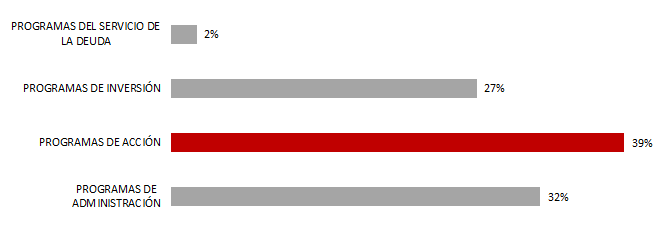
\includegraphics[width=14.5cm]{20181119_PresupuestoTotal2017.png}
    \caption{Representación porcentual del Presupuesto Total de la Municipalidad de Asunción discriminado por los programas para el año 2017. [Fuente: Portal de la Municipalidad de Asunción - Ejercicio Fiscal 2017]}
    \label{fig:porcentajePresupuesto}
\end{figure}

\begin{figure}[H]
    \centering
    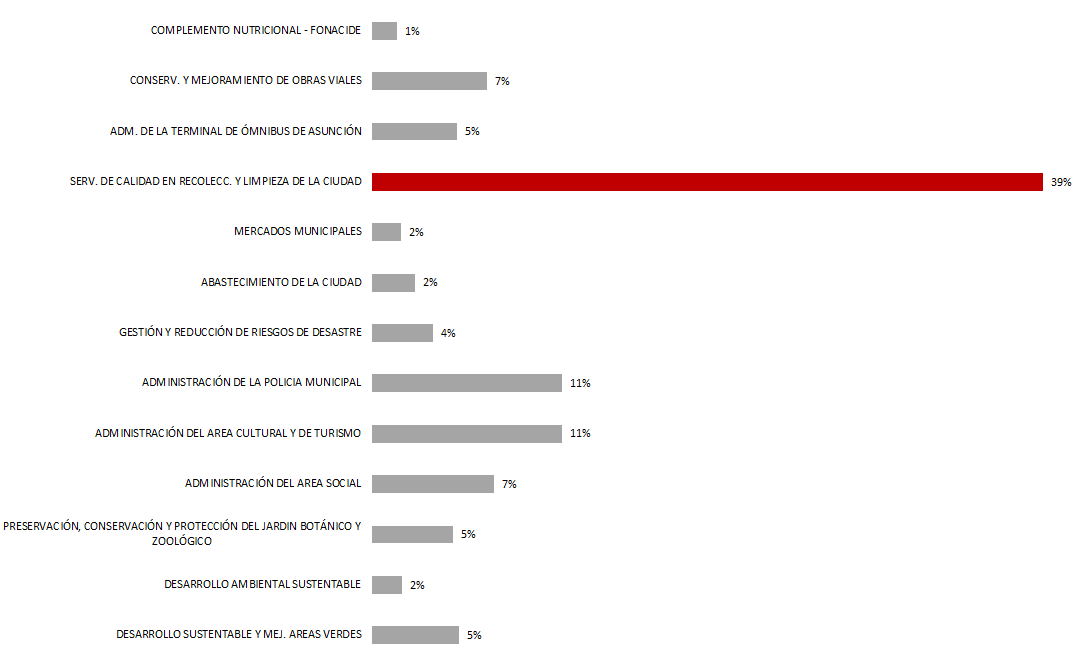
\includegraphics[width=15cm]{20181119_PresupuestoAccion2017.png}
    \caption{ Representación porcentual del Presupuesto correspondiente a los subprogramas del Programa de Acción correspondientes al año 2017. [Fuente: Portal de la Municipalidad de Asunción - Ejercicio Fiscal 2017]}
    \label{fig:programaAccion}
\end{figure}

Cuando se habla de la problemática de la gestión de residuos sólidos, es sabido que existen numerosos estudios y trabajos científicos que se han realizado al respecto con el propósito de resolverla usando objetivos económicos y/o ambientales como criterios para la toma de decisiones. Hasta hoy día se estudian distintas técnicas que puedan permitir mejorar el proceso que conlleva esto. Según \citet{Tchobanoglous1993IntegratedIssues} no hay un conjunto universal de reglas que puedan aplicarse a todas las situaciones.

En \citet{VitorinodeSouzaMelare2017TechnologiesReview} se realiza una revisión de los diversos procesos relacionados a la gestión de residuos sólidos y los agrupa en seis categorías: la gestión de recogida, recorrido y transporte; gestión y seguimiento de contenedores; reciclaje de residuos sólidos y gestión de residuos electrónicos; administración pública y desarrollo sostenible; métodos de previsión y planificación; y determinación de sitios de disposición de residuos.

Por lo general, la gestión de recolección de residuos sólidos urbanos en los países en desarrollo se basa en la experiencia práctica y los métodos intuitivos. Éstos dan lugar a prácticas ineficientes y costosas, que afectan tanto a la salud pública como al medio ambiente.

La fase de recolección es un problema de ruteo de vehículo que muchas veces se presenta como un problema NP-hard, y suele exigir un alto consumo de recursos computacionales. Como solución, se han propuesto métodos exactos tales como la Programación Lineal Entera Mixta (MILP, \textit{Mixed Integer Linear Programming}) \citep{Vecchi2016ACollection}, algoritmos heurísticos como el Algoritmo Genético (GA, \textit{Genetic Algorithm}) \citep{Mohammed2017SolvingSolution}, algoritmos meta heurísticos como el Algorítmo de Búsqueda Hacia Atrás (BSA, \textit{Backtracking Search Algorithm}) \citep{Akhtar2017BacktrackingOptimization}.



Por ello, es importante mencionar que, muchas de nuestras ciudades no tienen informatizado ni mucho menos resuelto el problema de la recolección eficiente de la basura, por lo que hemos visto hasta la fecha.

\section{Justificación}
Se ha visualizado la necesidad de optimizar el proceso de recolección de residuos, reduciendo el costo y el tiempo de cada recorrido, así como un mejor control de la flota de camiones recolectores. A su vez, permitirá a la Municipalidad de Asunción gestionar de manera eficiente, a través de una aplicación, que ofrecerá información actualizada en línea.

No sólo los ciudadanos que residen en la ciudad de Asunción serán beneficiados con un servicio más eficiente, sino las miles de personas, mencionadas más arriba, que ingresan diariamente a la ciudad, ya que al reducir el tiempo del vehículo recolector en tránsito se reduce el tráfico generado por los mismos y los problemas de contaminación por los líquidos y gases que dejan a su paso.
Este proceso, permitirá al personal encargado de la recolección de residuos agilizar su trabajo ya que pasarán menos tiempo en el vehículo recolector, mejorando así su calidad de vida.

Por todo lo expuesto, se considera plenamente justificada la investigación y propuesta de solución de este trabajo de fin de carrera, pues nos permitirá como ciudadanos retribuir en parte al Estado los beneficios y conocimientos que hemos adquirido a través de nuestra carrera en la Universidad.

\section{Objetivo General}
El objetivo general de este trabajo de investigación es el de proponer una solución óptima para el enrutamiento de vehículos de recolección de basura domiciliaria de la Dirección de Aseo Urbano de Asunción.

\section{Objetivos Específicos}

Los objetivos específicos que se han trazado en este trabajo para lograr el objetivo general son:
\begin{itemize}
    \item \textbf{Identificar} los factores que influyen en la recolección domiciliaria de la Dirección de Aseo Urbano.
    \item \textbf{Aplicar un modelo matemático} de optimización que mejor se ajuste a las reglas del negocio del caso de estudio.
    \item Comparar resultados del algoritmo propuesto con el modelo matemático seleccionado.
    \item \textbf{Proponer y desarrollar un prototipo de aplicación GIS} que permita configurar los parámetros de entrada y despliegue la ruta óptima para cada zona de recolección.
\end{itemize}


\section{Organización del Trabajo}

El resto del trabajo se organiza de la siguiente manera:

\begin{itemize}
    \item En el \textbf{capítulo 2} se presentan los conceptos básicos que describen la gestión de residuos sólidos municipales y el caso de estudio Asunción.
    \item En el \textbf{capítulo 3} se presentan conceptos básicos sobre Sistemas de Información Geográfica y bases de datos espaciales.
    \item En el \textbf{capítulo 4} se presentan las distintas técnicas de optimización.    
    \item En el \textbf{capítulo 5} se plantea de manera formal el problema que se intenta resolver. Se explican las formulaciones utilizadas, así como una explicación detallada de la implementación de la herramienta. 
    \item En el \textbf{capítulo 6} se visualizan y se discuten los resultados de la propuesta.
    \item En el \textbf{capítulo 7}, se finaliza el trabajo de investigación presentando las conclusiones generales.    
\end{itemize}